\documentclass{scrreprt}
\usepackage[letterspace=150]{microtype}
\usepackage{tikz}
\usetikzlibrary{automata,positioning}
\SetTracking
  [ name         = XXXX,
    no ligatures = {f},
    outer spacing = {1000,,} ]
  { encoding = OT1,
    family   = *,
    series   = m,
    shape    = n }
  { }

\begin{document}
A \textls{BBB} A


\begin{tikzpicture}
\draw(0,0) -- node[anchor=west,text width=5cm]{\textls[200]{test}}(1,1);
\draw(0,0) -- node[anchor=west,text width=5cm]{a \textls[200]{test} A}(10,1);
\draw(0,0) -- node[anchor=west,text width=5cm]{\textls*[200]{test}}(5,1);
\end{tikzpicture}

\begin{tikzpicture}
\draw(0,0) -- node[anchor=west,text width=5cm]{\textls*{test}}(1,1);
% The following reported by \contributor Daniel Dumke <daniel\at dumke.me>
% http://tug.org/pipermail/tex-live/2013-July/034007.html
\node[rotate=-270] at (0.646,4.683) {\lsstyle Supply};
\end{tikzpicture}

% The following reported by \contributor Christian Stark <cstark\at gmx.de>
%                 2009/07/28, MID: <7d81lgF2ad3ckU1@mid.dfncis.de>
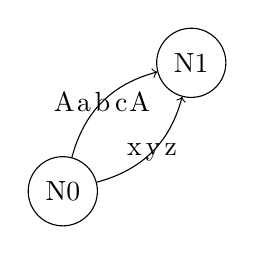
\begin{tikzpicture}
\node[state] (N0) {N0};
\node[state] (N1) [above right=of N0] {N1};
\path[->,bend left] (N0) edge node {A\textls{abc}A} (N1);
\path[->,bend right] (N0) edge node {\lsstyle xyz} (N1);
\end{tikzpicture}

A \textls{BBB} A

\end{document}

